\documentclass{whutmod}
\usepackage{metalogo}
\usepackage{float}
\usepackage{url}
\usepackage[style=caspervector,backend=biber,utf8]{biblatex}
\addbibresource{文献数据库.bib}
\team{38}	% 组号
\membera{李耘凡、刘子川}
\joba{编程}
\memberb{侯绍博、梁艺璇}
\jobb{建模}
\memberc{汪嘉屹、张聪}
\jobc{建模}

\title{基于聚类分析与非线性回归的ARIMA模型预测天然气负荷}
\tihao{1} % 题号

\begin{document}
	
	\maketitle
	
	\begin{abstract}
   本文在聚类分析的基础上通过ARIMA模型分析预测天然气负荷,采用灰色关联分析天气因素影响天然气用量的规律,最后采用非线性回归将天气因素加入到ARIMA模型中进行修正,对模型进行了优化改进。
~\\

   针对问题一,通过聚类分析将月份分为三类,对每一类分别建立ARIMA模型。采用SPSS专家建模法,得到了每个月份的天然气用量估计值,并进行模型检验,发现预测结果良好。
~\\

   针对问题二,通过ACF、PACF图进行模型识别,用AIC系数定阶,选择ARIMA(0,1,5)模型建模。利用Python进行数据预处理和可视化,并进行预测,得到该地区2016年3月23日9:00——4月11日8:00每小时总用气量。发现用气量以24小时为周期呈现出较强的周期性,一个月内的天然气销售量总体呈现波动下降趋势。并用均方根误差RMSE进行检验,对结果进行了合理性说明。
~\\

   针对问题三,引入经过量化处理的天气因素,采用灰色关联分析对天气因素进行分析,得到最低气温、最高气温、天气情况均与用气量相关联。计算出问题二中已有模型的预测数据与实际数据的差值序列,再建立差值序列关于天气因素的非线性回归模型,以此来预测修正值$y$,并对修正值非线性模型进行合理性检验。最后将修正值$y$与第二问ARIMA模型预测结果求和,即为新的预测。
~\\

   针对问题四,分为短期预测和长期预测,对短期预测进行分析可认为短期内经济、人口、季节等因素变化不大,可视为常量处理。同问题三的思路确定变量的相关关系。对于中长期预测,采用在时间序列的基础上综合多维线性回归模型得到结果。
~\\

   本文的优点有两点:一是使用聚类分析把月份合理化分组,使得预测精度得到提高;二是将天气影响因素采用较合理方法量化,降低了求解难度。


	
		
		\keywords{聚类分析\quad  ARIMA模型\quad   灰色关联分析\quad  非线性回归}
	\end{abstract}
	
	%目录
	\tableofcontents
	\newpage	%换页符
	
	\section{问题重述}
	\subsection{问题的背景}
		我国传统能源以石油、煤炭这两种重污染化石为主,经济的快速发展以破坏生态环境为代价。我国政府为了调整能源消费结构,出台了一系列政策措施。充分利用天然气这一环保清洁的能源,是解决经济发展与环境保护之间矛盾的有效途径。可以预见,天然气的需求量和消费量将逐年上升。天然气是石油和煤炭的优质替代品,但是我国天然气生产不能满足消费需求\parencite{鞠武2014中国天然气市场供需趋势研究}。天然气市场处于高速发展阶段,要保持天然气市场的持续稳定发展,分析天然气市场的供需平衡显得急迫而必要。合理预测某地区的天然气负荷量,是合理规划管道调度之前的重要环节,同时为未来国家政策的制定提供参考。
	
		天然气作为一种洁净环保的优质能源在工业和人们日常起着至关重要的作用。然而天然气在我国能源消费结构中占比不大,并且天然气产供储销体系还不完备,产业发展不平衡不充分问题较为突出,主要是国内产量增速低于消费增速,进口多元化有待加强,消费结构不尽合理,基础设施存在短板等问题,解决这些问题的前提就是要对天然气符合做出合理精确的预测,这对天然气负荷预测技术研究提出了高要求。对天然气负荷的合理预测无论对天然气供气系统的优化设计和运行还是我国可持续性发展都起着关键作用。如果没有基于经济社会、气象数据、人们生活习惯等因素的天然气的合理预测,会带来不必要的经济损失,造成浪费。而精确并快速的预测天然气负荷有利于应对天然气消费的季节性特点所导致天然气供应紧张出现“气荒”的问题\parencite{孙相博2019基于改进灰色}。所以合理并精确预测天然气负荷显得尤为重要,本文中根据天然气公司2014年A市小时用气量表,预测基于天然气用气量、经济社会、气象数据、生活习惯等因素有关的同期天然气消费需求的用气量改变的趋势。。
	
	\subsection{问题概述}
	
	围绕天然气负荷预测,依次提出如下问题:
	
	\begin{itemize}
		\item 根据2014年每小时的历史数据分析并预测该公司A市2015年每月销售情况;
		\item 根据历史数据分析并预测某地区2016年3月23日9:00——4月11日8:00每小时总用气量;
		\item 根据气象数据,考虑气象因素分析并预测某地区2016年3月23日9:00——4月11日8:00每小时总用气量;
		\item 深入考虑季节、经济增长、人口变化等其他因素的影响,对问题二的模型进行调整,并给出调整理由及调整后的模型。
	\end{itemize}
	
	\section{模型的假设}
	\begin{itemize}
		\item 假设每一年用气量呈周期性变化;
		\item 短期内该市的经济发展状况与人口数量不会出现大幅度的增长;
		\item 假设天气变化规律在两年内不变化;
		\item 假设天然气负荷量在某一年中季节性变动远大于长期趋势变动。
	\end{itemize}
	
	
	\section{符号说明}
	\begin{center}
		\begin{tabular}{cc}
			\hline
			\makebox[0.3\textwidth][c]{符号}	&  \makebox[0.4\textwidth][c]{意义} \\ \hline
			$p$	    & 自回归项数 \\ \hline
			$d$	    & 差分次数\\ \hline
			$q$	    & 移动平均项数 \\ \hline
		$\bigtriangledown ^{d}$ & 自回归系数多项式\\ \hline
		$\Theta (B)$ & 移动平滑系数多项式\\ \hline
			$y$	    & 非线性回归模型修正值  \\ \hline
		    $x1$	    & 最高气温 \\ \hline
		    		$x2$	    & 最低气温  \\ \hline
		    				$x3$	    & 天气情况量化数据 \\ \hline
		\end{tabular}
	\end{center}
	
	\section{问题一模型的建立与求解}
	\subsection{问题一描述与分析}
	%\subsubsection{问题一描述与分析}
	针对问题一,由于题中仅给出一年中该城市的用气量来预测下一年每月的用气量,并且数据没有一个很好的变化趋势进行拟合,我们不妨假设每一年的用气量呈现周期性变化,利用时间序列模型进行预测。又考虑到因季节、节假日等因素对用气量的影响,不同月份的变化趋势可能有较大区别,直接对一年的时间序列进行预测不合理,可以先将"距离"相近的月份进行聚类分类,即将变化趋势相同的月份分为一类,再分别进行预测,见流程图~\ref{aaa}~。
	\begin{figure}[H]
		\centering
		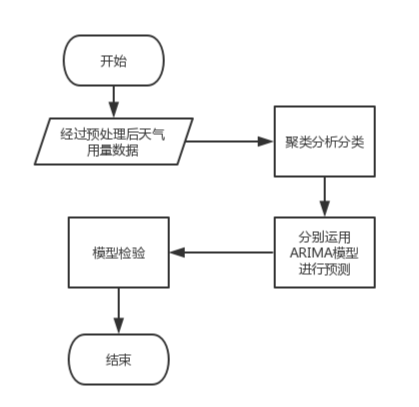
\includegraphics[width=.6\textwidth]{figures/aaa.png}
		\caption{问题一分析流程图}\label{aaa}
	\end{figure}
	%\subsubsection{模型建立与求解}
	\subsection{预备工作}
	我们首先将$2014$年每小时的天然气用量合并成每天的天然气用量,然后将其随天数的变化绘制成图,并将每个月的变化趋势分割,如图~\ref{img001}~所示。
	
	\begin{figure}[H]
		\centering
		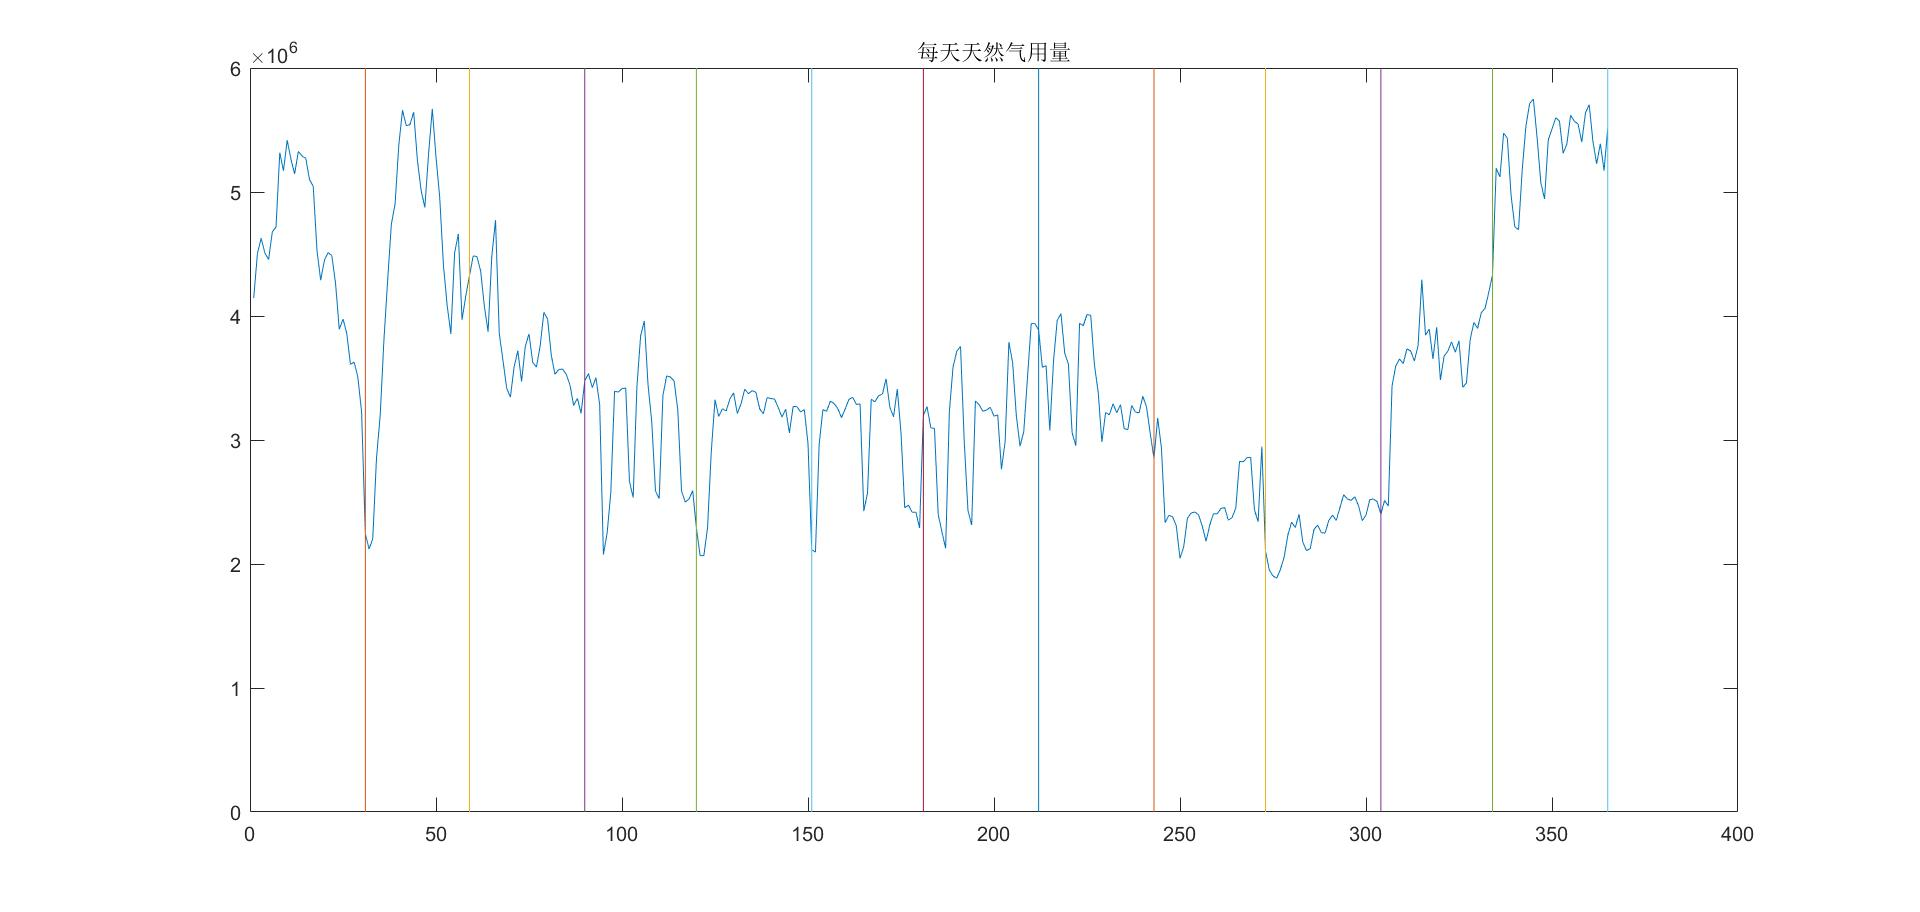
\includegraphics[width=\textwidth]{figures/1.jpg}
		\caption{2014年每月用气量变化趋势}\label{img001}
	\end{figure}
	
	观察图像可以得出$2014$年中,整体趋势处于紊乱状态,没有很好的周期性分布趋势,利用整体数据进行预测难以进行。因此,我们采取聚类分析的方法将12个月进行划分,找出相似的月份再分别运用ARIMA模型进行预测。
	%在$Minkowski$距离中,最常用的是欧几里得距离,它的主要优点是当坐标轴进行正交转换时,欧氏距离保持不变。其欧式距离定义如下:
	\subsection{模型的建立与求解}
	\subsubsection{聚类分析}
	在$Minkowski$距离中,最常用的是欧几里得距离,它的主要优点是当坐标轴进行正交转换时,欧氏距离保持不变。其欧式距离定义如下:
	\begin{gather*}
	%	gather(代编号) 和gather*(不代编号) 环境(可使用\\换行)
	d_{i}(x,y)=\left [ \sum_{k=1}^{p}|x_{k}-y_{k}|^{2} \right ]^{\frac{1}{2}}
	\end{gather*}
	式中x,y为来自用气量和时间的观测值。利用类与类的相似性度量它们之间的距离,当两类的欧氏距离很小时,它们能很好的各自聚为一类。其聚类图如图~\ref{img1}~所示,由图~\ref{img001}~和聚类结果表明,1、2月属于波动较大月份;$3\sim11$月属于波动较平缓月份;12月处于高消耗波动较平缓月份,我们可以将2014年的月份分为这三类部分,分别进行预测分析。
	
	\begin{figure}[H]
		\centering
		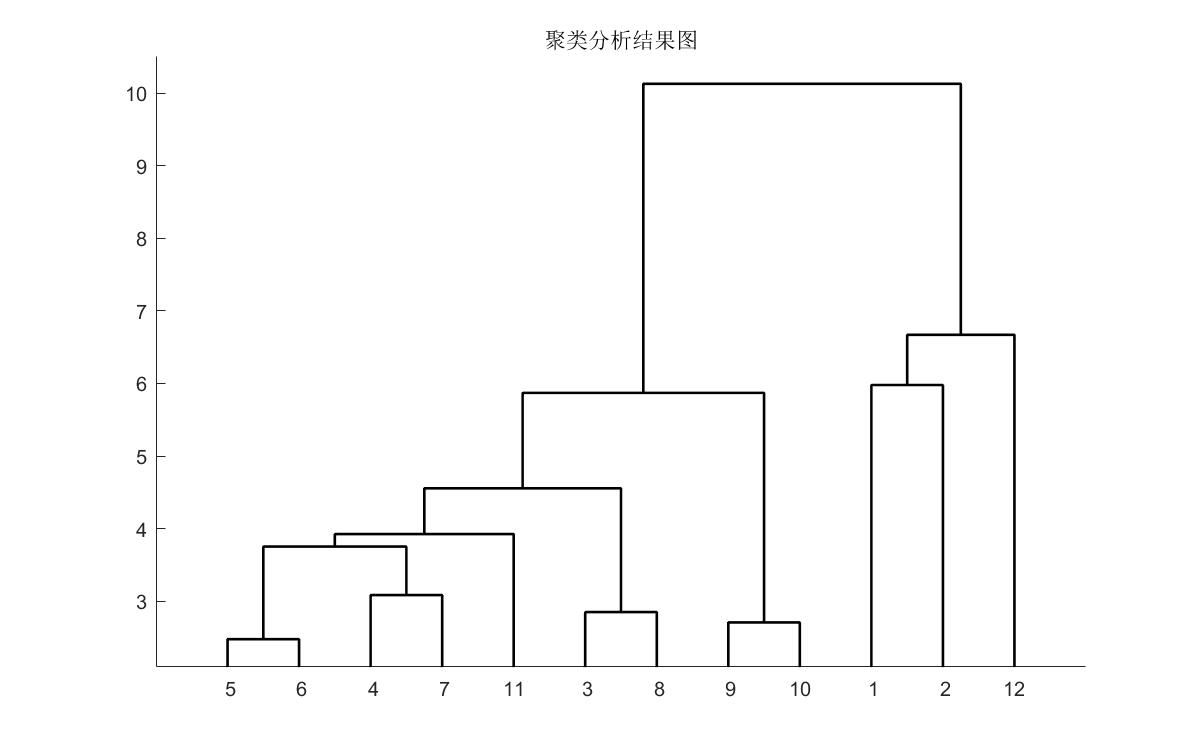
\includegraphics[width=.7\textwidth]{figures/untitled.jpg}
		\caption{聚类分析结果图}\label{img1}
	\end{figure}
	
	\subsubsection{问题一ARIMA模型}
	
	%针对上述聚类的每一类分别进行分析。绘制每日用气量折线图,发现波动较大,属于非平稳时间序列。先通过差分运算将非平稳时间序列转化为平稳序列,差分后出现非白噪声序列,再对差分后的序列建立ARIMA模型。
	ARIMA模型(差分整合移动平均自回归模型),简记为$ARIMA(p,d,q)$模型,是将非平稳时间序列经过差分运算转化为平稳时间序列后,再拟合ARIMA模型。ARIMA模型的结构如图~\ref{gs}~所示\parencite{conejo2005day}:
	\begin{figure}[H]
		\centering
		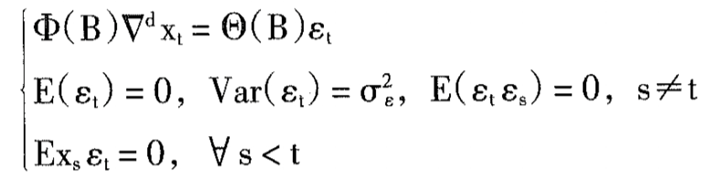
\includegraphics[width=.5\textwidth]{figures/gs.png}
		\caption{ARIMA模型的结构}\label{gs}
	\end{figure}
	式中,$\bigtriangledown ^{d}=(1-B)^{d}$,$\Phi \left ( B\right )= 1-\phi _{1}B-...-\phi _{p}B^{p}$为平稳可逆$ARMA(p,q)$模型的自回归系数多项式,$\Theta (B)=1-\theta _{1}B_{1}-...-\theta _{q}B_{q}$为平稳可逆序列$ARMA(p,q)$模型的移动平滑系数多项式\parencite{conejo2005day}。
	ARMA模型结构可以简记为:
	\begin{gather}
	\bigtriangledown^{d}x_{t}=\frac{\Theta (B)}{\Phi(B)}\varepsilon _{t}
	\end{gather}
	
	通过ARIMA模型的简化结构可以看出,ARIMA模型的实质就是差分运算和ARMA模型的结合。任何一个非平稳时间序列,如果可以通过适当阶数的差分运算实现平稳,就可以对差分平稳序列进行ARIMA模型的求解。
	
	经过聚类分析,1、2月份被分在一类中,首先对此类进行分析。我们直接利用SPSS软件对这一类的59天样本值进行时间序列分析,采取专家建模法得到如下结果:
	\begin{figure}[H]
		\centering
		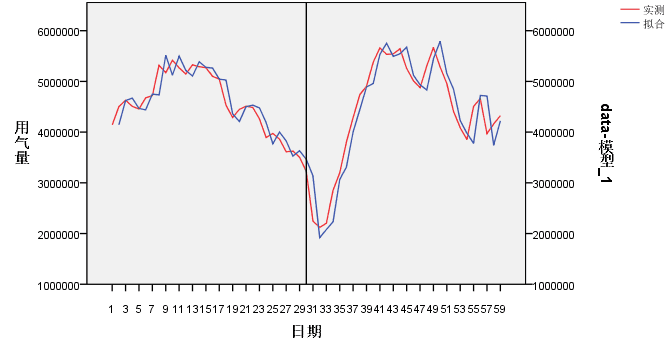
\includegraphics[width=\textwidth]{figures/a.png}
		\caption{第一类预测结果}\label{a}
	\end{figure}
	\begin{figure}[H]
		\centering
		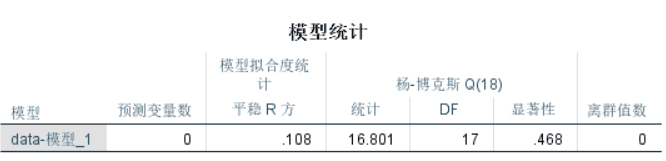
\includegraphics[width=.7\textwidth]{figures/a1.png}
		\caption{模型检验结果}\label{a1}
	\end{figure}
	
	由图~\ref{a}~可见,拟合程度较好。观察杨-博克斯检验的显著性水平值为0.468,通过显著性检验,如图~\ref{a1}~所示。此时模型为$ARIMA(1,0,2)$。%根据模型假设1中每一年的用气量呈周期性变化,可以预测2015年一月份与二月份的天然气值分别为$140058294.4$(方)和$124430252$(方),详见表~\ref{tab000}~
	
	同理可对其他两类月份组进行预测,模型分别为$ARIMA(1,0,3)$,$ARIMA(0,0,1)$,并且都通过检验。其结果如下图所示:
	
	\begin{figure}[H]
		\begin{minipage}[t]{0.45\linewidth}
			\centering
			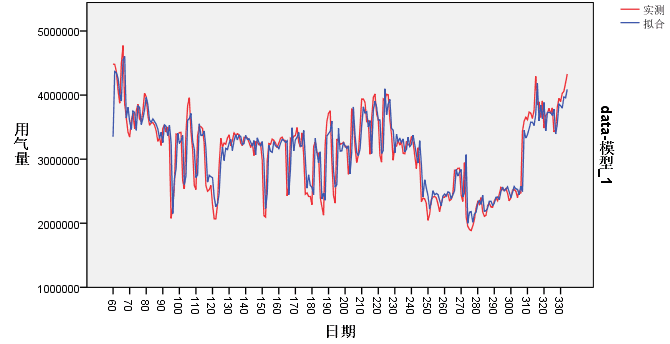
\includegraphics[width=\textwidth]{figures/b.png}
			\caption{第二类预测结果}
		\end{minipage}%
		\begin{minipage}[t]{0.45\linewidth}
			\centering
			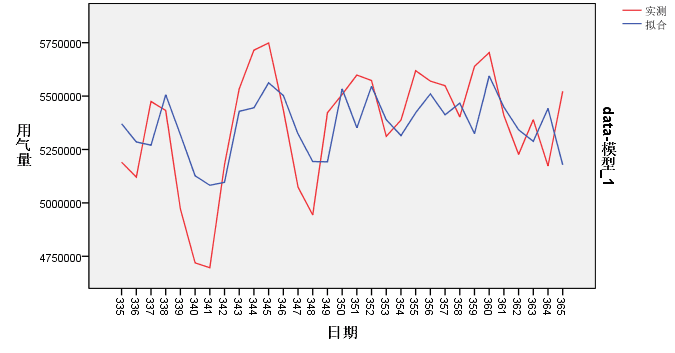
\includegraphics[width=\textwidth]{figures/c.png}
			\caption{第三类预测结果}
		\end{minipage}
	\end{figure}
	
	根据模型假设1中每一年的用气量呈周期性变化,不妨利用2014年的预测值代替2015年的用气量,得到结果如表~\ref{tab000}~所示
	\begin{table}[H]
		\caption{2015年每月用气量预测值(方)}\label{tab000} \centering
		\begin{tabular}{ccccc}
			\toprule[1.5pt]
			一月 & 二月 & 三月 & 四月 \\
			\hline
			140058294.4&124430252&116683453&94167977\\
			\hline
			五月 & 六月 & 七月&八月\\
			\hline
			93639575&94096616&97524051&106754917\\
			\hline
			九月 & 十月 &十一月 & 十二月 \\
			\hline
			77046944&72832081&107219489&166267451\\
			\bottomrule[1.5pt]
		\end{tabular}
	\end{table}
	
	%\subsection{问题二 ARMA模型}
	\section{问题二模型的建立与求解}
	\subsection{问题二描述和分析}
针对问题二,由于数据量较少,且只需要考虑时间因素,不必考虑其他影响因素,我们可以选择时间序列对其进行分析。时间序列分析方法采用基于自相关函数的最小二乘法建立天然气负荷AR模型,但这种方法不能充分利用天然气随季节、日期类型等因素呈现周期性变化的信息\parencite{刘涵2004基于最小二乘支持向量机的天然气负荷预测},所以采用ARIMA模型,考虑到求解过程的精确性,不再使用专家建模法。首先,我们需要检验序列的平稳性,选择合适的$p,q$模型,然后对自相关函数和偏相关函数图分析对模型进行定阶。再对模型进行检验,最终通过ARIMA模型得得到预测数据。
	\subsection{预备工作}
	我们首先将数据画图,如图~\ref{img003}~所示。发现前23天每小时的天然气消费量呈现出以24小时为周期的周期性,属于典型的时间序列问题。我们考虑时间序列分析,通过建立AIRMA模型,对历史数据进行模拟,并预测未来七天每小时的天然气负荷量。
	\begin{figure}[H]
		\centering
		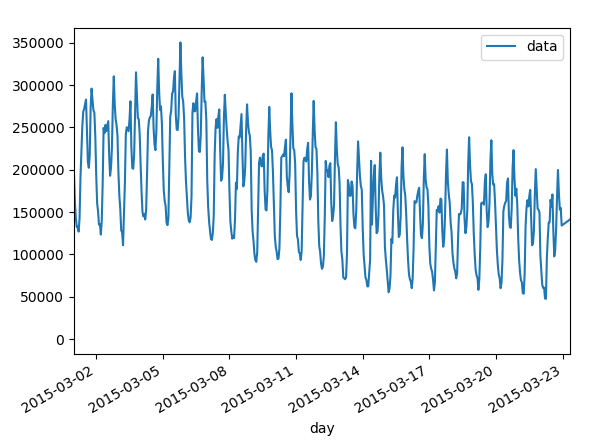
\includegraphics[width=.45\textwidth]{figures/3.png}
		\caption{2015年三月每小时的用气量}\label{img003}
	\end{figure}	
	\subsection{模型建立与求解}
	\paragraph{平稳性检验}
	
	为了检验时间序列的平稳性,可以运用图示法和根检验法\parencite{刘罗曼2010时间序列平稳性检验}。图示法即通过观察时序图的均值和方差,来判断时间序列的平稳性。这种方法主观性较强,可能会有一定的偏差。为了提高精确度,我们通过根检验法对事件进行平稳性检验,得到的结果如表~\ref{tab001}~所示,很明显数据序列不满足平稳性要求。
	
	\begin{table}[H]
		\caption{天然气负荷序列ADF检验结果}\label{tab001} \centering
		\begin{tabular}{ccccc}
			\toprule[1.5pt]
			检验标准 & 结果 \\
			\midrule[1pt]
			Test Statistic & -1.285790 \\
			p-value & 0.635648 \\
			Number of observations Used & 508 \\
			Critical value 1\% & -3.44 \\
			Critical value 5\% & -2.86 \\
			Critical value 10\% & -2.57 \\
			\bottomrule[1.5pt]
		\end{tabular}
	\end{table}
	
	\paragraph{序列差分操作}
	由于数据序列不满足平稳性要求,我们对数据序列做差分操作,使其满足平稳性要求,其中基本思想用流程图表示出来,如图~\ref{img004}~所示。
	
	\begin{figure}[H]
		\centering
		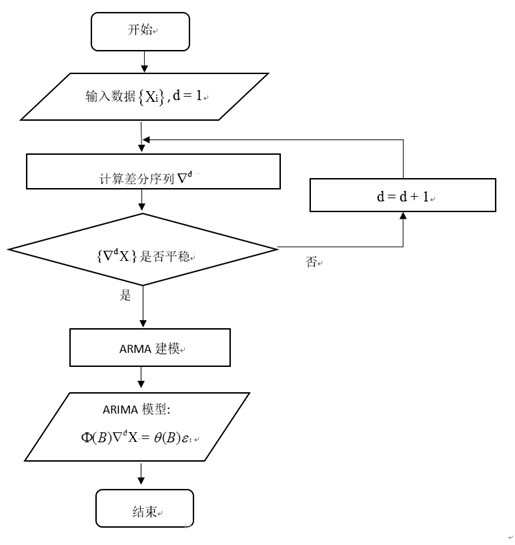
\includegraphics[width=.55\textwidth]{figures/4.jpg}
		\caption{差分操作的流程图}\label{img004}
	\end{figure}
	d是对原时序进行逐期差分的阶数,差分的目的时为了让某些非平稳序列变换成平稳的,通常来说d的取值一般为0,1,2
	差分操作的检验结果如表~\ref{tab003}~所示,一阶和二阶差分的对比如图~\ref{img006}~所示:
	\begin{table}[H]
		\caption{天然气负荷序列差分操作后ADF检验结果}\label{tab003} \centering
		\begin{tabular}{ccccc}
			\toprule[1.5pt]
			检验标准 & 结果\\
			\midrule[1pt]
			Test Statistic & $-1.073378e+01$ \\ 
			p-value & $2.934167e-19$ \\
			Number of observations Used & $4.860000e+02$ \\
			Critical value 1\% & $-3.443877e+00$ \\
			Critical value 5\% & $-2.867505e+00$ \\
			Critical value 10\% & $2.569947e+00$ \\
			\bottomrule[1.5pt]
		\end{tabular}
	\end{table}
	\begin{figure}[H]
		\centering
		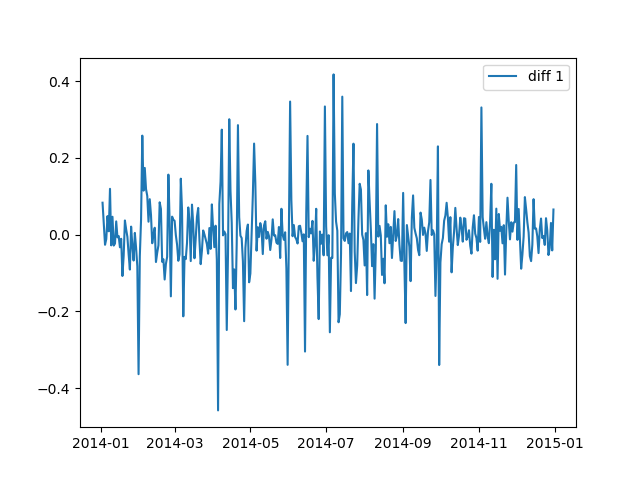
\includegraphics[width=.6\textwidth]{figures/6.png}
		\caption{一阶差分图}\label{img006}
	\end{figure}
	由检验结果和差分后数据图可知,一阶差分后的序列已经满足平稳性要求。
	\paragraph{模型识别} 
	
依据自相关函数图和偏向关函数图截尾与拖尾,来进行模型识别,如果序列相关系数拖尾,偏自相关系数$p$阶拖尾,选择$AR$;如果自相关系数$q$阶截尾,选择$MA$;如果自相关系数和偏相关系数均拖尾,选择$ARIMA$进行预测。\parencite{wang2015improving}
	
	自相关系数与偏自相关系数计算如图~\ref{img005}~所示:
	\begin{figure}[H]
		\centering
		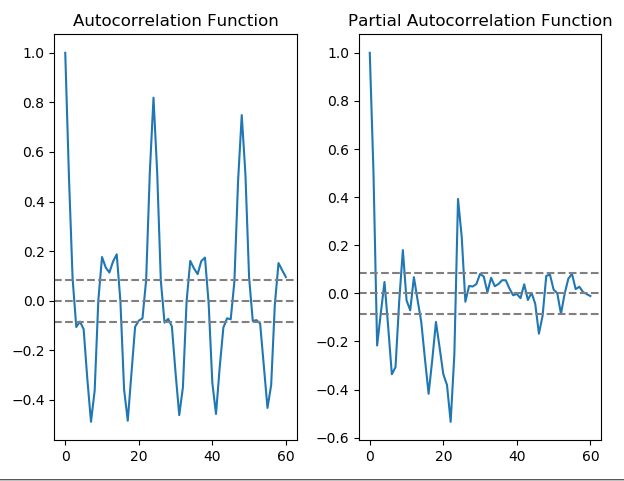
\includegraphics[width=.6\textwidth]{figures/5.png}
		\caption{自相关系数与偏自相关系数计算图}\label{img005}
	\end{figure}
由图可知自相关函数与偏向关函数均拖尾,故采用ARIMA模型进行预测。
	
	\paragraph{模型定阶} 所谓定阶,就是确定当前数据到底跟过去几天数据有关,这一步,同时选定模型,根据自相关、偏自相关函数的截尾、拖尾情况选定模型,其中过去几天数据的系数由偏相关系数决定,噪声系数由自相关系数决定\parencite{zhang2019prediction}。具体选取需要计算各选定模型的AIC值,选取最小AIC对应的模型,作为最终模型。
	
	简化自回归综合移动模型后得的表达式如下:
	\begin{gather}
	%	gather(代编号) 和gather*(不代编号) 环境(可使用\\换行)
	AIC(p,q) = 2(p+q)-2ln(L)
	\end{gather}
	
	公式中,$p=0,q=5$分别表示AR模型和MA模型的阶数,L表示ARIMA模型的极大自然数。其模型如图~\ref{img009}~所示
	\begin{figure}[H]
		\centering
		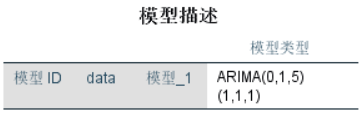
\includegraphics[width=.5\textwidth]{figures/9.png}
		\caption{建立的模型}\label{img009}
	\end{figure}
	\paragraph{预测结果}
	
	利用python进行数据预处理和可视化之后,我们将数据导入到SPSS中,利用自带的时间序列预测工具进行计算,最后得到模型类型为$ARIMA(0,1,5)(1,1,1)$,并且是随季节性变化,其预测该地区三月每小时用气量如图~\ref{img007}~所示,详细预测结果见附录。
	
	\begin{figure}[H]
		\centering
		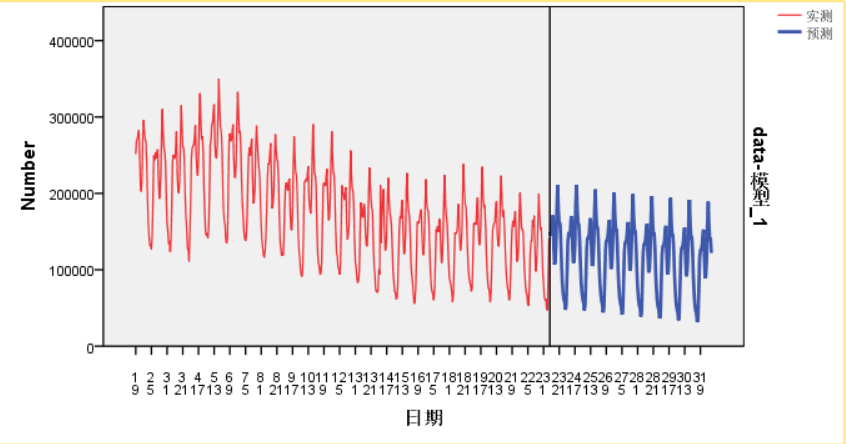
\includegraphics[width=\textwidth]{figures/7.png}
		\caption{该地区三月每小时总用气量}\label{img007}
	\end{figure}
	\paragraph{模型检验}
	对于模型预测性能的评价,主要考察的是模型预测值与实际值之间的大小,不同的评价指标可以从不通的角度反映模型的预测能力。因为没有拿其他模型进行比较,根据自身的检验,我们利用均方根误差进行检验$RMSE = \sqrt{\frac{1}{N}\sum_{i=1}^{N}(Y_{i}-\overline{Y}_{i})}$。我们的主要关切是确保我们的模型的残差是不相关的,并且平均分布为零。我们的模型诊断表明,模型残差正常分布如图~\ref{img0010}~所示。
	
	\begin{figure}[H]
		\centering
		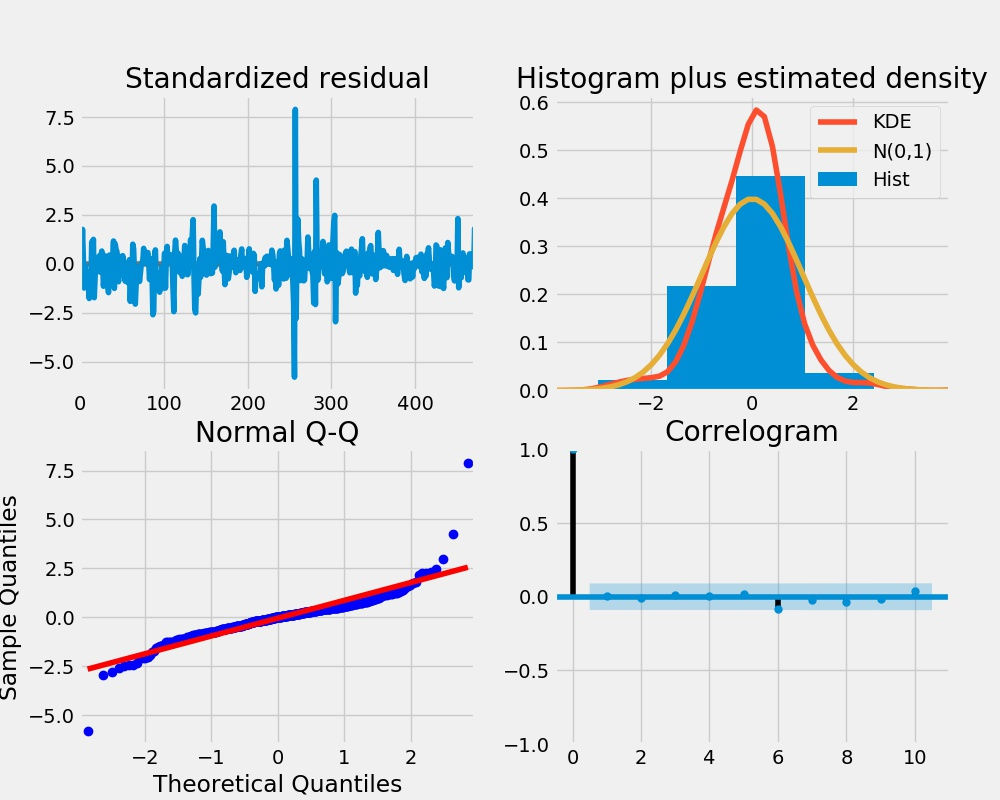
\includegraphics[width=.6\textwidth]{figures/111.jpg}
		\caption{模型统计与诊断}\label{img0010}
	\end{figure}
	
	随着时间的推移的残差不会显示任何明显的季节性,似乎是白噪声。 这通过右下角的自相关图来证实,这表明时间序列残差与其本身的滞后版本具有低相关性。这些观察结果使我们得出结论,该模型可以帮助我们了解时间序列数据和预测未来价值。

	由于不考虑季节、经济增长、人口变化等其他因素对天然气用气量的影响,根据模型的模拟与预测,我们可以得出:
	\begin{itemize}
		\item 一天的用气高峰出现在中午1点左右以及晚上七点左右
		\item 一个月内的天然气消费量总体呈现波动下降趋势,以24小时为周期呈现出较强的周期性
	\end{itemize}
	
	
	\section{问题三模型的建立与求解}
	\subsection{问题描述和分析}
对于问题三,要求在问题二的基础上加入天气因素建立模型进行重新预测,我们考虑到在问题2建立的ARIMA模型上加以改进来做出新的预测。首先,我们需要分析出影响较为显著的天气因素来作为模型的数据,因此我们采用灰色关联分析先对天气因素的影响做出分析。然后,计算出问题2中已有模型对已知时间点的预测数据与实际数据的差值序列。最后,建立差值序列关于天气因素的回归模型,通过回归模型计算出修正值重新预测。
	\subsection{预备工作}
	将问题2中预测3月1日至3月22日天然气用量的差值以及三种天气因素数据进行标准化。
	将天气情况指标量化处理,如表~\ref{tabycl}~所示:
	\begin{table}[H]
	\caption{天气情况指标量化处理}\label{tabycl} \centering
	\begin{tabular}{ccccc}
		\toprule[1.5pt]
		晴 & 多云 & 阴 & 阵雨 \\
		\hline
		1&2&3&4\\
		\hline
		小雨 & 中雨 & 大雨&暴雨\\
		\hline
		5&6&7&8\\
		\hline
		雨夹雪 & 小雪 &中雪 \\
		\hline
		9&10&11\\
		\bottomrule[1.5pt]
	\end{tabular}
	\end{table}
	其中,高转低表示为:$(max+min)/2-0.1$,
	低转高表示为:$(max+min)/2+0.1$ 。
	\subsection{模型建立与求解}
	
	\subsubsection{灰色关联分析}
	由于考虑到用气量受多个天气因素的影响,我们采取灰色关联分析来分析各个因素对于结果的影响程度,根据分析结果来选择回归模型中的自变量,灰色关联分析是指对一个系统发展变化态势的定量描述和比较的方法,其基本思想是通过确定参考数据列和若干个比较数据列的几何形状相似程度来判断其联系是否紧密,它反映了曲线间的关联程度。首先对每个特征确定分析数列并做归一化,再进行关联系数\parencite{刘思峰2013灰色关联分析模型研究进展},其公式如下:
	
	\begin{gather}
		\xi _{i}\left ( k \right )=\frac{min_{i} min_{k}\Delta _{i}(k)+\rho max_{i} max_{k}\Delta _{i}(k)}{\Delta _{i}(k)+\rho max_{i} max_{k}\Delta _{i}(k)}
	\end{gather}
	
	
	式中记$\Delta _{i}(k)=|y(k)-x_{i}(k)|$,$\rho \in (0,\infty )$称为分辨系数。$\rho $越小,分辨力越大,一般$\rho $的取值区间为(0,1),具体取值可视情况而定。当$\rho \leqslant  0.5463$时,分辨力最好,通常取$\rho =0.5$。
	对各评价对象(比较序列)分别计算其个指标与参考序列对应元素的关联系数的均值,以反映各评价对象与参考序列的关联关系,依据各观察对象的关联序,得出分析结果如下图所示:
	\begin{figure}[H]
	\begin{minipage}[t]{0.5\linewidth}
		\centering
		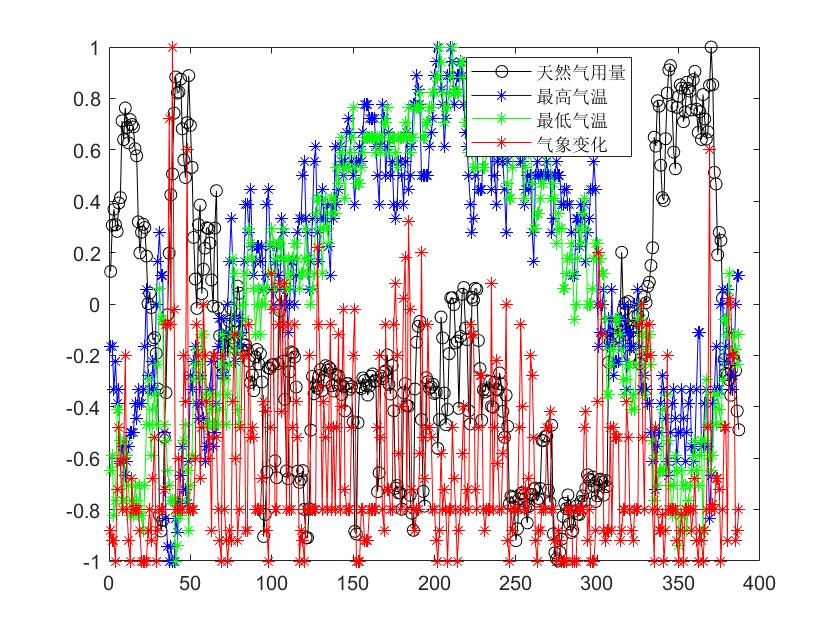
\includegraphics[width=\textwidth]{figures/gld1.jpg}
		\caption{标准化后对比图}
	\end{minipage}%
	\begin{minipage}[t]{0.5\linewidth}
		\centering
		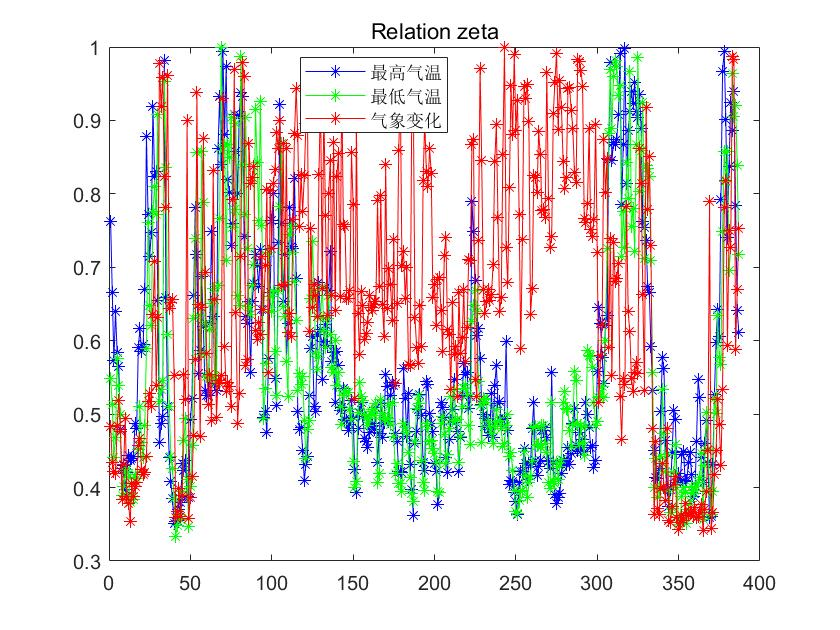
\includegraphics[width=\textwidth]{figures/gld2.jpg}
		\caption{灰色关联系数}
	\end{minipage}

	得到最高气温,最低气温,天气情况三个特征的$\rho $分别为0.5678、0.5596、0.6675,分辨力均较好,即都与用气量相关联。因此在回归模型中同时考虑3种天气因素。
\end{figure}
	\subsubsection{非线性回归模型}
	首先,将天然气用量差值,最高气温,最低气温,天气情况绘制差值序列变化趋势图初步确定经验公式。
	\begin{figure}[H]
		\centering
		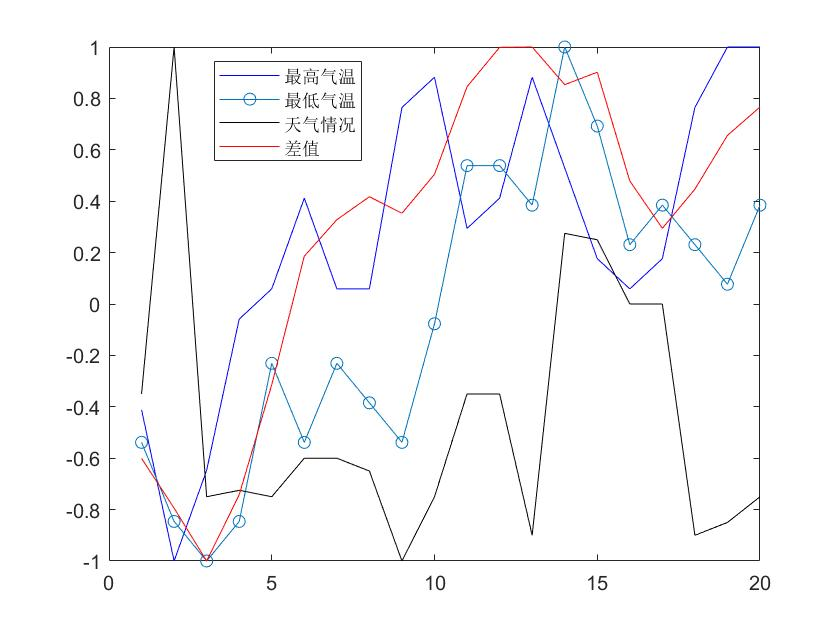
\includegraphics[width=\textwidth]{figures/hgfx1.jpg}
		\caption{自变量与因变量变化对比图}\label{img003}
	\end{figure}	
	由图~\ref{img003}~可知,差值序列与天气因素未呈现出明显的线性关系,考虑使用非线性二次回归模型。求解结果如下图所示:
		\begin{figure}[H]
			\centering
			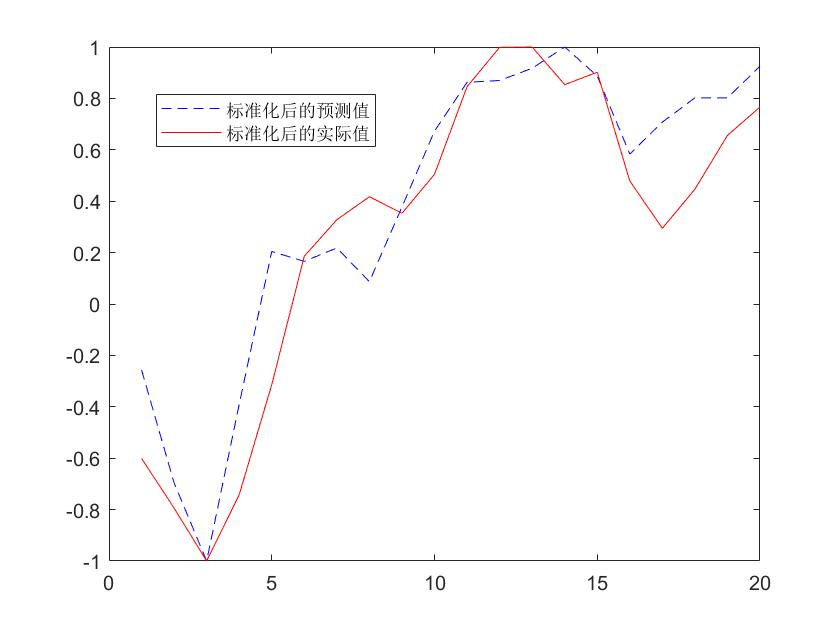
\includegraphics[width=\textwidth]{figures/hgfx2.jpg}
			\caption{非线性回归模型预测差值对比图}\label{img003}
		\end{figure}	
		非线性回归方程为 :
			\begin{gather}
		y =a + b*x_{1}*x_{2} + c*x_{1}*x_{3} +d*x_{2}*x_{3} + e*x_{3}^2
			\end{gather}
			式中$x1$,$x2$,$x3$分别表示最高气温,最低气温与天气情况。
各项系数的求解结果见附录。对此非线性回归模型进行检验,结果如下表:
	
	\begin{table}[H]
		\caption{非线性回归模型检验结果}\label{tab001} \centering
		\begin{tabular}{ccccc}
			\toprule[1.5pt]
			检验标准 & 结果 \\
			\midrule[1pt]
		R-squared & 0.889 \\
		Adjusted R-Squared& 0.825 \\
		 p-value & $7.1e-05$\\
			\bottomrule[1.5pt]
		\end{tabular}
	\end{table}
	由模型假设2,天气变化规律在短期内不变化,可以将2014年的3月23日至4月11日的天气指标作为2015年对应的日期的天气因素指标。又因为非线性回归模型是根据天数来建立修正值的,我们将其取平均作为小时的修正值。
	因此,将此非线性回归模型得到的差值$y$取24等份作为每小时的修正值,再与问题2中建立的ARIMA模型的预测值叠加便得到了修正后的预测值,预测对比图如下,具体数值见附录。
		\begin{figure}[H]
			\centering
			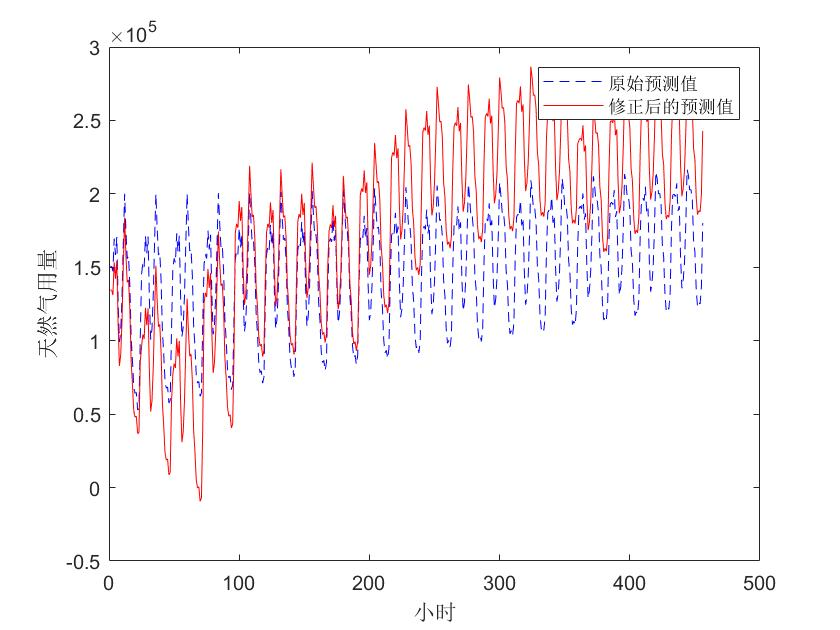
\includegraphics[width=\textwidth]{figures/hgfx3.jpg}
			\caption{预测对比图}\label{img003}
		\end{figure}	
由上图可知修正后的预测值呈现出向上波动的趋势。	
	\section{问题四的调整模型}
	
	深入考虑季节、经济增长、人口变化等其他因素对天然气用气量的影响,对问题的模型进行调整。	由于在较短时间内季节变化因素影响不大,经济增长缓慢的增长,一个城市的人口增长也是平稳的,故对于天然气负荷的短期预测可以将经济、人口、季节等因素视为常量。但是对于天然气的中长期预测,它们的动态变化对于天然气的消费量的影响起到了不可忽视的作用。故而我们调整模型时,可分为两种情形。
	
	\subsection{短期预测}
	由于客观事物的内在规律的复杂性和人们认识程度的限制,无法分析实际对象内在的因果关系,而利用第三问中的回归模型确定的变量之间的相关关系,会表现出一定的规律性,因此不需要进行调整。
	\subsection{中长期预测}
	ARIMA模型只针对于时间变元进行分析,无法综合考虑其他因素的影响,故而我们采用多维度回归模型对其进行一定的调节。使之既保有原始时间序列的周期性与趋势性,也添加进其他因素的影响。
	
	我们在时间序列的基础上综合多维线性回归模型。设$x_{i}$为时间序列,则有:
	\begin{center}
		%		内容...
		
		\begin{gather}
			\left\{  
			\begin{aligned}  
				Z(1)=p_{0}+p_{1}x_{11}+p_{2}x_{12}+\xi _{1} &  \\  
				Z(2)=p_{0}+p_{1}x_{21}+p_{2}x_{22}+\xi _{2} & \\
				............................. & \\  
				Z(n)=p_{0}+p_{1}x_{n1}+p_{2}x_{n2}+\xi _{n}&    
			\end{aligned}  
			\right.  
		\end{gather}
	\end{center}
	
	其中,该市人口数为$x_{1}$,经济总量为$x_{2}$,季节为$x_{3}$,$p_{i}$为影响变量的待定系数,$\xi _{i}$用于控制模型中的随机性。
	\section{模型的评价}
	\subsection{模型的优点}
	本文在考虑未来一年的用气量预测时时,按照月份分类进行分析;确定不同类别的月份后,对不同ARIMA模型进行预测。在第二问的模型求解时,由于存在季节性的变化,本文利用内生变量进行模型的定阶与识别进一步增强了模型的可靠性,而不是进行复杂的网格搜索进行调参,最终得到理想的最优结果。 并且在考虑温度、天气等因素的影响时,没有重新建立新模型进行预测,而采取对问题二中的结果与实际值进行残差分析,利用非线性回归拟合出预测的曲线,并在原模型上进行多维度的调整。
	
	\subsection{模型的缺点}
	在考虑预测2015年数据的时候,由于没有收集到完整数据,本文假设了年份呈周期性变化,忽略经济增长、人口变化、国情等其他因素的影响,考虑欠妥当。利用问题二预测的数据进行残差分析时,实际略不相符,故存在缺陷。

	
	
	\newpage	%换页符
	%%参考文献
	%\begin{thebibliography}{9}%宽度9
	% \setlength{\itemsep}{-2mm}
	
	\printbibliography[title = {参考文献}]	%使用国标参考文献添加方式
	
	% \bibitem{bib:one} 
	% 韩中庚. 数学建模方法及其应用[M]. 高等教育出版社, 2005.
	% \bibitem{bib:two}
	% 韩中庚. 数学建模方法及其应用[M]. 高等教育出版社, 2005.
	% \bibitem{bib:two}
	% 韩中庚. 数学建模方法及其应用[M]. 高等教育出版社, 2005.
	% 
	% \nocite{*}		%排版未引用的参考文献
	% \bibliography{文献数据库}	%不同书库用数据分割
	%
	%\end{thebibliography}
	
	\newpage
	%附录
	\appendix %%附录
	\section{代码}
	\subsection{数据提取与合并--matlab 源程序}
	\begin{lstlisting}[language=matlab]
sj0=xlsread('附件1.xlsx','C6:C8765');
%以小时,天,月为时间单位,总共365天
%创建用于spss时间序列分析的数据
%sj0是原始数据集,先合并成天再合并成月
sjd=zeros(365,1);%合并成天
%xlswrite('第一问数据(年).xlsx',sj0);
for i=1:1:365%以天为单位
t1=24*(i-1)+1;
t2=24*i;
s=0;
sjd(i,1)=sum(sj0(t1:1:t2));
end
sjm=zeros(12,1);%以月份为单位
sjm(1)=sum(sjd(1:31));%一月

%%
sjm(2)=sum(sjd(32:59));%二月
sjm(3)=sum(sjd(60:90));%三月
sjm(4)=sum(sjd(91:120));%四月
sjm(5)=sum(sjd(121:151));
sjm(6)=sum(sjd(152:181));
sjm(7)=sum(sjd(182:212));
sjm(8)=sum(sjd(213:243));
sjm(9)=sum(sjd(244:273));
sjm(10)=sum(sjd(274:304));
sjm(11)=sum(sjd(305:334));
sjm(12)=sum(sjd(335:365));
%xlswrite('第一问数据(月度).xlsx',sjm);
figure
plot(sjd);
hold on%绘制竖线标注
%y1=max(sjd);
y1=6*10^6;
plot([31,31],[0,y1]);%1
plot([59,59],[0,y1]);%2
plot([90,90],[0,y1]);%3
plot([120,120],[0,y1]);%4
plot([151,151],[0,y1]);%5
plot([181,181],[0,y1]);%6
plot([212,212],[0,y1]);%7
plot([243,243],[0,y1]);%8
plot([273,273],[0,y1]);%9
plot([304,304],[0,y1]);%10
plot([334,334],[0,y1]);%11
plot([365,365],[0,y1]);%12
xlabel('天数'),ylabel('天然气用量');
figure
plot(sjm)
%xlswrite('第一问数据 (天).xlsx',sjd);
%不考虑综合分析,先对每个月的数据进行分析
figure
plot(sjd)
figure
subplot(2,6,1),plot(sjd(1:31));
subplot(2,6,2),plot(sjd(32:59));
subplot(2,6,3),plot(sjd(60:90));
subplot(2,6,4),plot(sjd(91:120));
subplot(2,6,5),plot(sjd(121:151));
subplot(2,6,6),plot(sjd(152:181));
subplot(2,6,7),plot(sjd(182:212));
subplot(2,6,8),plot(sjd(213:243));
subplot(2,6,9),plot(sjd(244:273));
subplot(2,6,10),plot(sjd(274:304));
subplot(2,6,11),plot(sjd(305:334));
subplot(2,6,12),plot(sjd(335:365));
sjm12=[sjd(335:365)];
xlswrite('12月数据',sjm12)
sjm122=[sjd(1:31);sjd(32:59)];
xlswrite('1,2月数据',sjm122);
sjmqt=[sjd(60:334)];
xlswrite('中间类别月份的数据',sjmqt);
%xlswrite('2,6月的数据',sjm26)
sjm45=[sjd(91:120);sjd(121:151);sjd(182:212);sjd(244:273)];
%xlswrite('4,5月等的数据',sjm45);
figure
plot(sjd(1:31));
\end{lstlisting}
\subsection{聚类分析程序--matlab源代码}
\begin{lstlisting}[language=matlab]

clc,clear
%%聚类分析原始数据生成(取值30天)
sj0=xlsread('附件1.xlsx','C6:C8765');
sjd=zeros(365,1);
for i=1:1:365%以天为单位
t1=24*(i-1)+1;
t2=24*i;
s=0;
sjd(i,1)=sum(sj0(t1:1:t2));
end
gj=zeros(12,30);
for i=1:1:12
gj(i,:)=(sjd(((i-1)*30+1):1:i*30))';
end
gj=zscore(gj); %数据标准化
y=pdist(gj); %求对象间的欧氏距离,每行是一个对象
z=linkage(y,'average');  %按类平均法聚类
h=dendrogram(z);
title('聚类分析结果图')%画聚类图
set(h,'Color','k','LineWidth',1.3)  %把聚类图线的颜色改成黑色,线宽加粗
for k=3:5
fprintf('划分成%d类的结果如下:\n',k)
T=cluster(z,'maxclust',k);  %把样本点划分成k类
for i=1:k
tm=find(T==i);  %求第i类的对象
tm=reshape(tm,1,length(tm)); %变成行向量
fprintf('第%d类的有%s\n',i,int2str(tm)); %显示分类结果
end
if k==5
break
end
fprintf('**********************************\n');
end
\end{lstlisting}

\subsection{灰色关联分析--matlab 源程序}
\begin{lstlisting}[language=matlab]
%% 数据预处理
%提取天气因素各项数据
clear
sj0=xlsread('附件2.xlsx','C6:C533');%合并附件二中的数据备用
%只需生成一次,加快运行速度
sj0d=zeros(22,1);
for i=1:1:22
t1=24*(i-1)+1;t2=24*i;
sj0d(i,1)=sum(sj0(t1:1:t2));
end
xlswrite('15年问题3',sj0d);%注意sjd不要加‘’
sj14=xlsread('14年问题3(天).xlsx','A1:A365');
sj15=xlsread('15年问题3.xls','A1:A22');
sj03=[sj14;sj15];
sj01=xlsread('附件1.xlsx','H3:I367');%提取2014最高气温最低气温
sj02=xlsread('附件2.xlsx','H3:I24');%2015气温数据
sj0=[sj01;sj02];
sj0=mapminmax(sj0');sj0=sj0';%mapminmax按行进行数据归一化
sj01=sj0(:,1);sj02=sj0(:,2);
sj03=mapminmax(sj03');sj03=sj03';
sj011=xlsread('附件1天气情况.xlsx','B1:B365');%提取气象变化数据
sj012=xlsread('附件2天气情况.xlsx','B1:B22');
sj00=[sj011;sj012];
sj00=mapminmax(sj00');sj00=sj00';
%% 进行灰色关联分析
%sj03存储天然气用量归一化数据,sj01储存最高气温
%sj02储存最低气温
% define comparative and reference
x0=sj03';
x1=sj01';%最高气温因素
x2=sj02';%最低气温因素
x3=sj00';%气象变化因素
%初值归一化,本程序使用初值归一化
%x0 = x0 ./ x0(1);
%x1 = x1 ./ x1(1);
%x2 = x2 ./ x2(1);
%x3 = x3 ./ x3(1);
% global min and max
global_min = min(min(abs([x1; x2;x3] - repmat(x0, [3, 1]))));
global_max = max(max(abs([x1; x2;x3] - repmat(x0, [3, 1]))));
% set rho
rho = 0.5;
% calculate zeta relation coefficients
%灰色关联系数计算公式
zeta_1 = (global_min + rho * global_max) ./ (abs(x0 - x1) + rho * global_max);
zeta_2 = (global_min + rho * global_max) ./ (abs(x0 - x2) + rho * global_max);
zeta_3 = (global_min + rho * global_max) ./ (abs(x0 - x3) + rho * global_max);
%% 可视化处理
figure;
plot(x0, 'ko-' )
hold on
plot(x1, 'b*-')
hold on
plot(x2, 'g*-')
hold on
plot(x3, 'r*-')
legend('天然气用量', '最高气温', '最低气温','气象变化')
figure;
plot(zeta_1, 'b*-')
hold on
plot(zeta_2, 'g*-')
hold on
plot(zeta_3, 'r*-')
title('Relation zeta')
legend('最高气温', '最低气温', '气象变化')
%% 计算关联系数均值判断相关性
z1=mean(zeta_1)
z2=mean(zeta_2)
z3=mean(zeta_3)

\end{lstlisting}

\subsection{非线性回归分析--matlab 源程序}
\begin{lstlisting}[language=matlab]
clear
%% 数据准备
sj15s=xlsread('附件1.xlsx','C54:C533');%读取15年22天每小时的实际数据
%3月2日10点为起始点,从3月3日开始提取数据,只有20天数据
%计算24小时的和值重新生成数据,保证输入数与输出数个数相同
sj15y=xlsread('data_df5.csv','A49:A528');%读取对应预测数据(SPSS求出)
sj15dy=zeros(20,1);
x=1:1:480;
figure
plot(x,sj15s,x,sj15y)
for i=1:1:20
sj15dy(i)=sum(sj15y((24*(i-1)+1):1:24*i));
end
sj15ds=zeros(20,1);
for i=1:1:20
sj15ds(i)=sum(sj15s((24*(i-1)+1):1:24*i));
end
sj15c=zeros(20,1);
sj15c=sj15ds-sj15dy;%计算残差序列(待拟合),因变量输出
sj01=xlsread('附件2.xlsx','H5:I24');%2015气温数据提取
sj02=xlsread('附件2天气情况.xlsx','B3:B22');%2015气温数据提取
%sjt=1:1:20;sjt=sjt';%加入时间变化自变量
sj15x=[sj01,sj02];%自变量集合20*3矩阵,每行代表一次输入
%% 数据归一化
%sj15x=mapminmax(sj15x');sj15x=sj15x';
%sj15c=mapminmax(sj15c');sj15c=sj15c';
%% 绘制残差序列图推断变化规律
figure
plot(sj15c);legend('残差序列图')

%% 尝试使用集成命令拟合
%自变量是sj15x 20*3矩阵
%因变量是sj15c 20*1矩阵
fxxhg=LinearModel.fit(sj15x,sj15c,'poly112')%非线性回归分析
%% 可视化
%绘制3个自变量与一个因变量的对比图
yczx=fxxhg.predict(sj15x)
figure
ycz=mapminmax(fxxhg.predict(sj15x)');ycz=ycz';
sjz=mapminmax(sj15c');sjz=sjz';
plot(ycz,'b--');
hold on
plot(sjz,'r-');
legend('标准化后的预测值','标准化后的实际值');
figure
x=1:1:20;
%先进行归一化
y1=sj15x(:,1);y2=sj15x(:,2);y3=sj15x(:,3);y4=sj15c;
y1=mapminmax(y1');y1=y1';
y2=mapminmax(y2');y2=y2';
y3=mapminmax(y3');y3=y3';
y4=mapminmax(y4');y4=y4';
plot(x,y1,'b-',x,y2,'o-',x,y3,'k-',x,y4,'r-')
legend('最高气温','最低气温','天气情况','差值')
%读取原始预测值
yc1=xlsread('data_df4.csv','A1:A456');
%修正预测值
%yczx(20)=[];
for i=1:1:19
for j=(1+24*(i-1)):1:(24*i)
ycz3(j,1)=yczx(i)./24;
end
end
yc2=ycz3+yc1;
x=1:1:456;
figure
plot(x,yc1,'b--',x,yc2,'r-');
xlabel('小时');ylabel('天然气用量')
legend('原始预测值','修正后的预测值')

\end{lstlisting}
\subsection{求解ARIMA模型--python源代码}
\begin{lstlisting}[language=python]import import numpy as np
import matplotlib.pylab as plt
from statsmodels.tsa.seasonal import seasonal_decompose
from statsmodels.tsa.stattools import acf, pacf
from statsmodels.tsa.arima_model import ARIMA
from statsmodels.graphics.tsaplots import plot_acf, plot_pacf
from statsmodels.tsa.stattools import adfuller

def clear_data():
#数据加载
data = pd.read_csv('./demo2.csv', encoding='utf-8')
time = data["time"]
data = data["data"]

i=0
x={}
day=1
while i <data.size:
x["2015-3-" + str(day)+" "+str(time[i])] = data[i]
i+=1
if((i+1)%24==0):
day=day+1

observed = pd.DataFrame(list(x.items()), columns=['day','data'])
observed.to_csv('data_df2.csv', index=False, header=True)
observed.set_index("day", inplace=True)
observed.index = pd.DatetimeIndex(observed.index)
print(observed)

return observed
# 移动平均图
def draw_trend(timeseries, size):
f = plt.figure(facecolor='white')
# 对size个数据进行移动平均
rol_mean = timeseries.rolling(window=size).mean()
# 对size个数据移动平均的方差
rol_std = timeseries.rolling(window=size).std()

timeseries.plot(label='Original')
rol_mean.plot(color='red', label='Rolling Mean')
rol_std.plot(color='black', label='Rolling standard deviation')
plt.legend(loc='best')
# 绘制网格
plt.grid(alpha=0.2)
plt.title('Rolling Mean & Standard Deviation')
plt.xlabel("Date")
plt.ylabel("Used quantity")
plt.show()

def draw_moving(timeSeries, size):
f = plt.figure(facecolor='white')
# 对size个数据进行移动平均
rol_mean = timeSeries.rolling(window=size).mean()
# 对size个数据进行加权移动平均
rol_weighted_mean = pd.ewma(timeSeries, span=size)
# rol_weighted_mean=timeSeries.ewm(halflife=size,min_periods=0,adjust=True,ignore_na=False).mean()

timeSeries.plot(label='Original')
rol_mean.plot(color='red', label='Rolling Mean')
rol_weighted_mean.plot(color='black', label='Weighted Rolling Mean')
plt.legend(loc='best')
plt.title('Rolling Mean')
plt.xlabel("Date")
plt.ylabel("Used quantity")
plt.show()

# 自相关和偏相关图,默认阶数为31阶
def draw_acf_pacf(ts, lags=31):
f = plt.figure(facecolor='white')
ax1 = f.add_subplot(211)
plot_acf(ts, lags=31, ax=ax1)
ax2 = f.add_subplot(212)
plot_pacf(ts, lags=31, ax=ax2)
plt.show()

def test_stationarity(timeseries):
# 决定起伏统计
rolmean = timeseries.rolling(24).mean()  # 在某点取之前的12个做平均
rolstd = timeseries.rolling(24).std()  # 在某点取之前的12个算标准差
# 画出起伏统计
orig = plt.plot(timeseries, label='Original')
mean = plt.plot(rolmean, color='red', label='Rolling Mean')
std = plt.plot(rolstd, color='black', label='Rolling Std')
plt.legend(loc='best')
plt.title('Rolling Mean & Standard Deviation')
plt.show(block=False)
# 进行df测试
print('Result of Dickry-Fuller test')
dftest = adfuller(timeseries, autolag='AIC')
dfoutput = pd.Series(dftest[0:4], index=['Test Statistic', 'p-value', '#Lags Used', 'Number of observations Used'])
for key, value in dftest[4].items():
dfoutput['Critical value(%s)' % key] = value
print(dfoutput)

if __name__ == "__main__":
observed =clear_data()
print(observed.axes)
draw_trend(observed,24)

ts_log = np.log(observed)
# teststationarity(observed)
# draw_moving(ts_log, 24)

# estimating
ts_log = np.log(observed["data"])  #对数变换
moving_avg = ts_log.rolling(24).mean()
ts_log_moving_avg_diff = ts_log - moving_avg
ts_log_moving_avg_diff.dropna(inplace=True)
test_stationarity(ts_log_moving_avg_diff) #看数据是否具有平稳性
plt.show()
#
ts_log_diff = ts_log.diff(1)  # 1阶差分
ts_log_diff.dropna(inplace=True)
test_stationarity(ts_log_diff)
plt.show()
#
ts_log_diff1 = ts_log.diff(1)  #对比2阶差分
ts_log_diff2 = ts_log_diff1.diff(1)
plt.plot(ts_log_diff1, label='diff 1')
plt.plot(ts_log_diff2, label='diff 2')
plt.legend(loc='best')
plt.show()

# 分解decomposing
decomposition = seasonal_decompose(ts_log_diff)

trend = decomposition.trend  # 趋势
seasonal = decomposition.seasonal  # 季节性
residual = decomposition.resid  # 剩余的

plt.subplot(411)
plt.plot(ts_log,label='Original')
plt.legend(loc='best')
plt.subplot(412)
plt.plot(trend,label='Trend')
plt.legend(loc='best')
plt.subplot(413)
plt.plot(seasonal,label='Seasonarity')
plt.legend(loc='best')
plt.subplot(414)
plt.plot(residual,label='Residual')
plt.legend(loc='best')
plt.tight_layout()
plt.show()

#确定参数
lag_acf = acf(ts_log_diff, nlags=60)
lag_pacf = pacf(ts_log_diff, nlags=60, method='ols')
plt.subplot(121)
plt.plot(lag_acf)
plt.axhline(y=0, linestyle='--', color='gray')
plt.axhline(y=-1.96 / np.sqrt(len(ts_log_diff)), linestyle='--', color='gray')  # lowwer置信区间
plt.axhline(y=1.96 / np.sqrt(len(ts_log_diff)), linestyle='--', color='gray')  # upper置信区间
plt.title('Autocorrelation Function')
plt.subplot(122)
plt.plot(lag_pacf)
plt.axhline(y=0, linestyle='--', color='gray')
plt.axhline(y=-1.96 / np.sqrt(len(ts_log_diff)), linestyle='--', color='gray')
plt.axhline(y=1.96 / np.sqrt(len(ts_log_diff)), linestyle='--', color='gray')
plt.title('Partial Autocorrelation Function')
plt.tight_layout()
plt.show()

ts_log = ts_log.asfreq(None)

#     #选取参数0,1,4
model = ARIMA(ts_log, order=(0, 1, 4))
result_ARIMA = model.fit(disp=-1)
# print(result_ARIMA.fittedvalues)
pred = result_ARIMA.predict('2015-03-23 08:00:00','2015-04-11 08:00:00',dynamic=True)
# pred_ci = result_ARIMA.conf_int()
print("****"+pred.head(10))
# print(pred_ci)
plt.plot(ts_log_diff)
plt.plot(result_ARIMA.fittedvalues, color='red')
plt.title('ARIMA RSS:%.4f' % sum(result_ARIMA.fittedvalues - ts_log_diff) ** 2)
plt.show()

predictions_ARIMA_diff = pd.Series(result_ARIMA.fittedvalues, copy=True)
print(predictions_ARIMA_diff.head())#发现数据是没有第一行的,因为有1的延迟

predictions_ARIMA_diff_cumsum = predictions_ARIMA_diff.cumsum()
print(predictions_ARIMA_diff_cumsum.head(10))

predictions_ARIMA_log = pd.Series(ts_log.ix[0], index=ts_log.index)
predictions_ARIMA_log = predictions_ARIMA_log.add(predictions_ARIMA_diff_cumsum, fill_value=0)
# print(predictions_ARIMA_log.head())

predictions_ARIMA = np.exp(predictions_ARIMA_log)
predictions_ARIMA.to_csv("predictions_ARIMA.csv")
print(predictions_ARIMA)
plt.plot(observed)
plt.plot(predictions_ARIMA)
plt.title('predictions_ARIMA RMSE: %.4f' % np.sqrt(sum((predictions_ARIMA - observed['data']) ** 2) / len(observed['data'])))
plt.show()
#
# predict_sunspots = result_ARIMA.predict('2015-03-23 8:00:00', '2015-03-31 8:00:00', dynamic=True)
# print(predict_sunspots)
# fig, ax = plt.subplots(figsize=(12, 8))
# ax = observed.ix['1927':].plot(ax=ax)
# fig = result_ARIMA.plot_predict('2015-03-23 8:00:00', '2015-03-31 8:00:00', dynamic=True, ax=ax, plot_insample=False)
# plt.show()


\end{lstlisting}


\end{document}